\section{Theoretical Background}

\newcommand{\Na}{\ensuremath{{}^{22} \mathrm{Na}} }
\newcommand{\Cs}{\ensuremath{{}^{137} \mathrm{Cs}} }

The following sections will give an overview of topics which are necessary
to explain the \compton effect and our equipment we use to measure the
effect. 

\subsection{Radioactive Sources}
In our experiment we use two different sources of radiation \Na and \Cs .

\vspace{1em}\textbf{Sodium-22 \cite{naPaper}:} We use \Na for the energy calibration and to set the delays. The \Na isotope undergoes a 
beta ($\beta^+$) decay as illustrated in equation (\ref{eq:betaP}).
\begin{align}
  {}^{22}_{11} \mathrm{Na} \longrightarrow {}^{22}_{10} \mathrm{Ne} + e^+ + \nu_e
  \label{eq:betaP}
\end{align}
A proton of the sodium decays to a neutron and the sodium therefore becomes neon.
To account to conservation of charge and lepton number a positron $e^+$
and an electron neutrino $\nu_e$ is emitted. The life time of \Na is 2.6 years.
The positron annihilates with surrounding electrons which creates two
photons with an energy of $511 \mathrm{keV}$ each. The produced neon is
in an excited state which returns to the ground state in a lifetime of
$5 \mathrm{ps}$ under emission of a photon with an energy of
$1275 \mathrm{keV}$.
It is also possible that the sodium undergoes electron capture
\begin{align}
  {}^{22}_{11} \mathrm{Na} + e^- \longrightarrow {}^{22}_{10} \mathrm{Ne} +
  \nu_e.
  \label{eq:ecap}
\end{align}
An electron from the K shell interacts with a proton of the nucleus which
becomes a neutron by emission of an anti-electron neutrino.  Other electrons
fill the hole in the K shell and thereby emit a photon.  The electron
capture is ten times less likely than beta decay. 


\vspace{1em}\textbf{Cesium-137 \cite{csPaper}:} We use \Cs for the
energy calibration, to show the conservation of energy and to measure the
differential cross section. The \Cs isotope undergoes a beta ($\beta^-$)
decay
\begin{align}
  {}^{137}_{55} \mathrm{Cs} \longrightarrow {}^{137}_{56} \mathrm{Ba} + e^-
  + \bar{\nu}_e.
  \label{eq:betaM}
\end{align}
A neutron of the cesium decays to a proton and the cesium therefore becomes barium.
To account to the conservation of charge and lepton number an electron $e^-$
and an anti-electron neutrino $\bar{\nu}_e$ is emitted. The life time of \Cs is 30 years.
The produced barium is in an excited state which returns to the ground state in a lifetime of
$2.5 \mathrm{min}$ under emission of a photon with an energy of $661.7 \mathrm{keV}$.
We will use these photons for our experiment.

\subsection{\compton Scattering}
The \compton scattering is an elastic scattering of a free electron and a
photon. Due to the photon we have to do a relativistic calculation. Let us
assume that the electron with mass $m_e$ is at rest and the incoming photon
$\gamma$ has the wavelength $\lambda = \frac{h}{E_\gamma}$ (we choose an unit
system with $c=1$). See figure \ref{fig:compton}.
\begin{figure}[tbp]
  \centering
  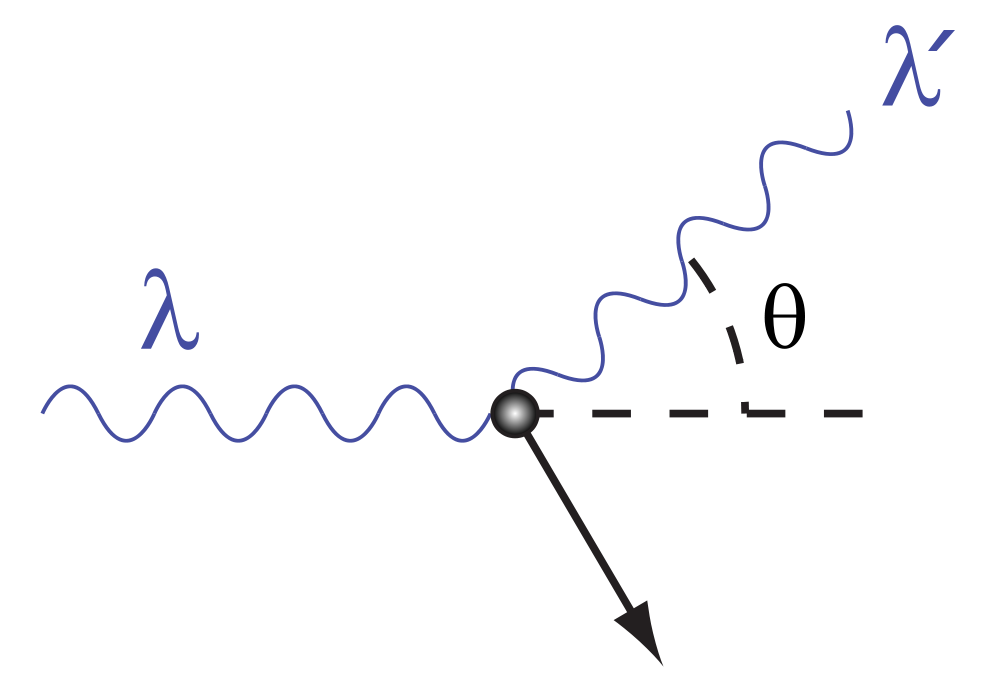
\includegraphics[width=0.5\textwidth]{Compton-scattering.png}
  \caption{Illustration of the \compton scattering. Source \cite{streuungBild}.}
  \label{fig:compton}
\end{figure}
The relativistic four-momenta in the lab system are
\begin{align}
  p_\gamma = \vecC{E_\gamma\\ E_\gamma \cdot \evec{e}_z}, \quad
  p_e = \vecC{m_e\\ \evec{0}}, \quad
  p'_\gamma = \vecC{E'_\gamma\\ E'_\gamma \cdot \evec{e}_f}
  \label{eq:fourMomenta}
\end{align}
where the primed quantities correspond to the quantities after the scattering.
The unit (three-)vectors $\evec{e}_z$ and $\evec{e}_f$ enclose the scattering angle
$\theta$, so $\evec{e}_z \cdot \evec{e}_f = \cos \theta$. 
We do not need to introduce the four-vector of the scattered electron.
The total energy is conserved, therefore
\begin{align}
  p_\gamma + p_e &= p'_\gamma + p'_e\\
  \Longrightarrow \quad  (p_\gamma + p_e - p'_\gamma)^2 &= {p'_e}^2.
  \label{eq:csDerivation1}
\end{align}
Evaluation the square and using the invariant square of the four-vectors
$p_\gamma^2 = {p'_\gamma}^2 = 0$ and $p_e^2 = {p'_e}^2 = m_e$, equation
(\ref{eq:csDerivation1}) yields
\begin{align}
  p_\gamma p_e &= p_e p'_\gamma + p_\gamma p'_\gamma \\
  \overset{(\ref{eq:fourMomenta})}{\Longleftrightarrow} \quad
  E_\gamma m_e &= E'_\gamma m_e + E_\gamma E'_\gamma - E_\gamma E'_\gamma \cos
  \theta \label{eq:csDerivation2}
\end{align}
From (\ref{eq:csDerivation2}) we can solve for $E'_\gamma$ and get
\begin{align}
  E'_\gamma = \frac{E_\gamma}{1 - \frac{E_\gamma}{m_e} (1-\cos \theta)} 
  \label{eq:egamma}
\end{align}
or we can plug in $E = \frac{h}{\lambda}$ and solve for the wave length shift
\begin{align}
  \lambda' - \lambda = \frac{h}{m_e} (1- \cos \theta)
\end{align}
which is the famous result that \compton derived. From (\ref{eq:egamma}) we
can calculate the energy of the scattered electron
\begin{align}
  E'_e = E_\gamma - E'_\gamma = E_\gamma \cdot \left( 1- \frac{1}{1 -
  \frac{E_\gamma}{m_e} (1-\cos \theta)}\right)
  \label{eq:eelectron}
\end{align} 

Besides \compton scattering there are other interactions of light with
matter. Photons can decay into a electron-positron pair, what is called pair
production. For that, the photons need to have at least an energy of $E=2\cdot
m_e=1.022\mathrm{MeV}$. The photons from the \Cs source do not have enough
energy to produce these pairs. An other interaction is called
photo electrical effect. Here the photon ionizes an atom. According to
\cite{dem4} \compton scattering is the most dominant effect for photons with
$E=662\mathrm{keV}$. We will compensate the influence of the photo electrical
when we calculate the differential cross section.

\subsection{Scintillator}
Scintillators are used to detect ionizing radiation, utilizing that certain organic
and inorganic materials emit light, when exposed to radiation.
This light can be detected with a photomultiplier. In general a scintillator
consists of a scintillating material and a photomultiplier.

%The function can be explained with the band-model, using the energy of the incoming electromagnetic radiation, energy is assigned to the scintillator material, so electrons can switch from the valence band to the conduction band. Under emission of electromagnetic radiation they fall back to ground state. There has to be different energy levels so the secondary radiation will not be absorbed immediately. For anorganic scintillators the crystal gets contaminated, for organic scintillators is a frequency pusher used to create different excitation energies.

\subsubsection{Organic Scintillator}
Organic scintillators are made of organic materials, the one in our
experiment is a PVC scintillator. The scintillating material absorbs photons or
charged particles what causes excites molecules. When the molecules relax,
they emit light. There are added wave length shifters, to make the
scintillator transparent for the scintillation light. 

In our experiment the \compton scattering takes place inside the organic
scintillators. The scattered electrons are detected here, whereas the
scattered photons are supposed to leave the organic scintillator.

\subsubsection{Inorganic Scintillator}
Inorganic scintillators are contaminated crystals. Here the ionized
radiation produces electron-gap pairs, which operate as charge carrier. When
they fall back into the ground state, they emit light. At some places the
conduction band is deformed, what changes the energy level. This makes the
scintillator transparent for the scintillator light.

We use a sodium iodide (NaI) scintillator, to detect the photons, which
are scattered inside the plastic scintillator.

\newcommand{\kleinn}{\person{Klein-Nishina}}

\subsection{Cross Section}
The cross section describes the probability that an interaction takes place.
The total cross section states the probability that an
interaction takes place in general, the differential cross section, the one
we will measure in our experiment, states the probability that an
interaction takes place in a defined solid angle.

The cross section depends on the energy of the scattered and scattering
particles and on the impact parameter.  For \compton scattering the
theoretical differential cross section can be expressed with the \kleinn  formula
\begin{align}
 \tder{\sigma}{\Omega} = \frac{1}{2} r^2_e E'_{\gamma} (\theta) (1 -
 E'_{\gamma} (\theta) sin^2 (\theta) + E'_{\gamma} (\theta) ).
 \label{eq:kleinn}
\end{align}
$E_{\gamma}$ is the same as in equation (\ref{eq:egamma}). For further
information on this see \cite{otto}. The
differential cross section is shown in figure \ref{fig:kleinn}. The 
\kleinn  formula is to be verified in our experiment. 

\begin{figure}[tbp]
  \centering
  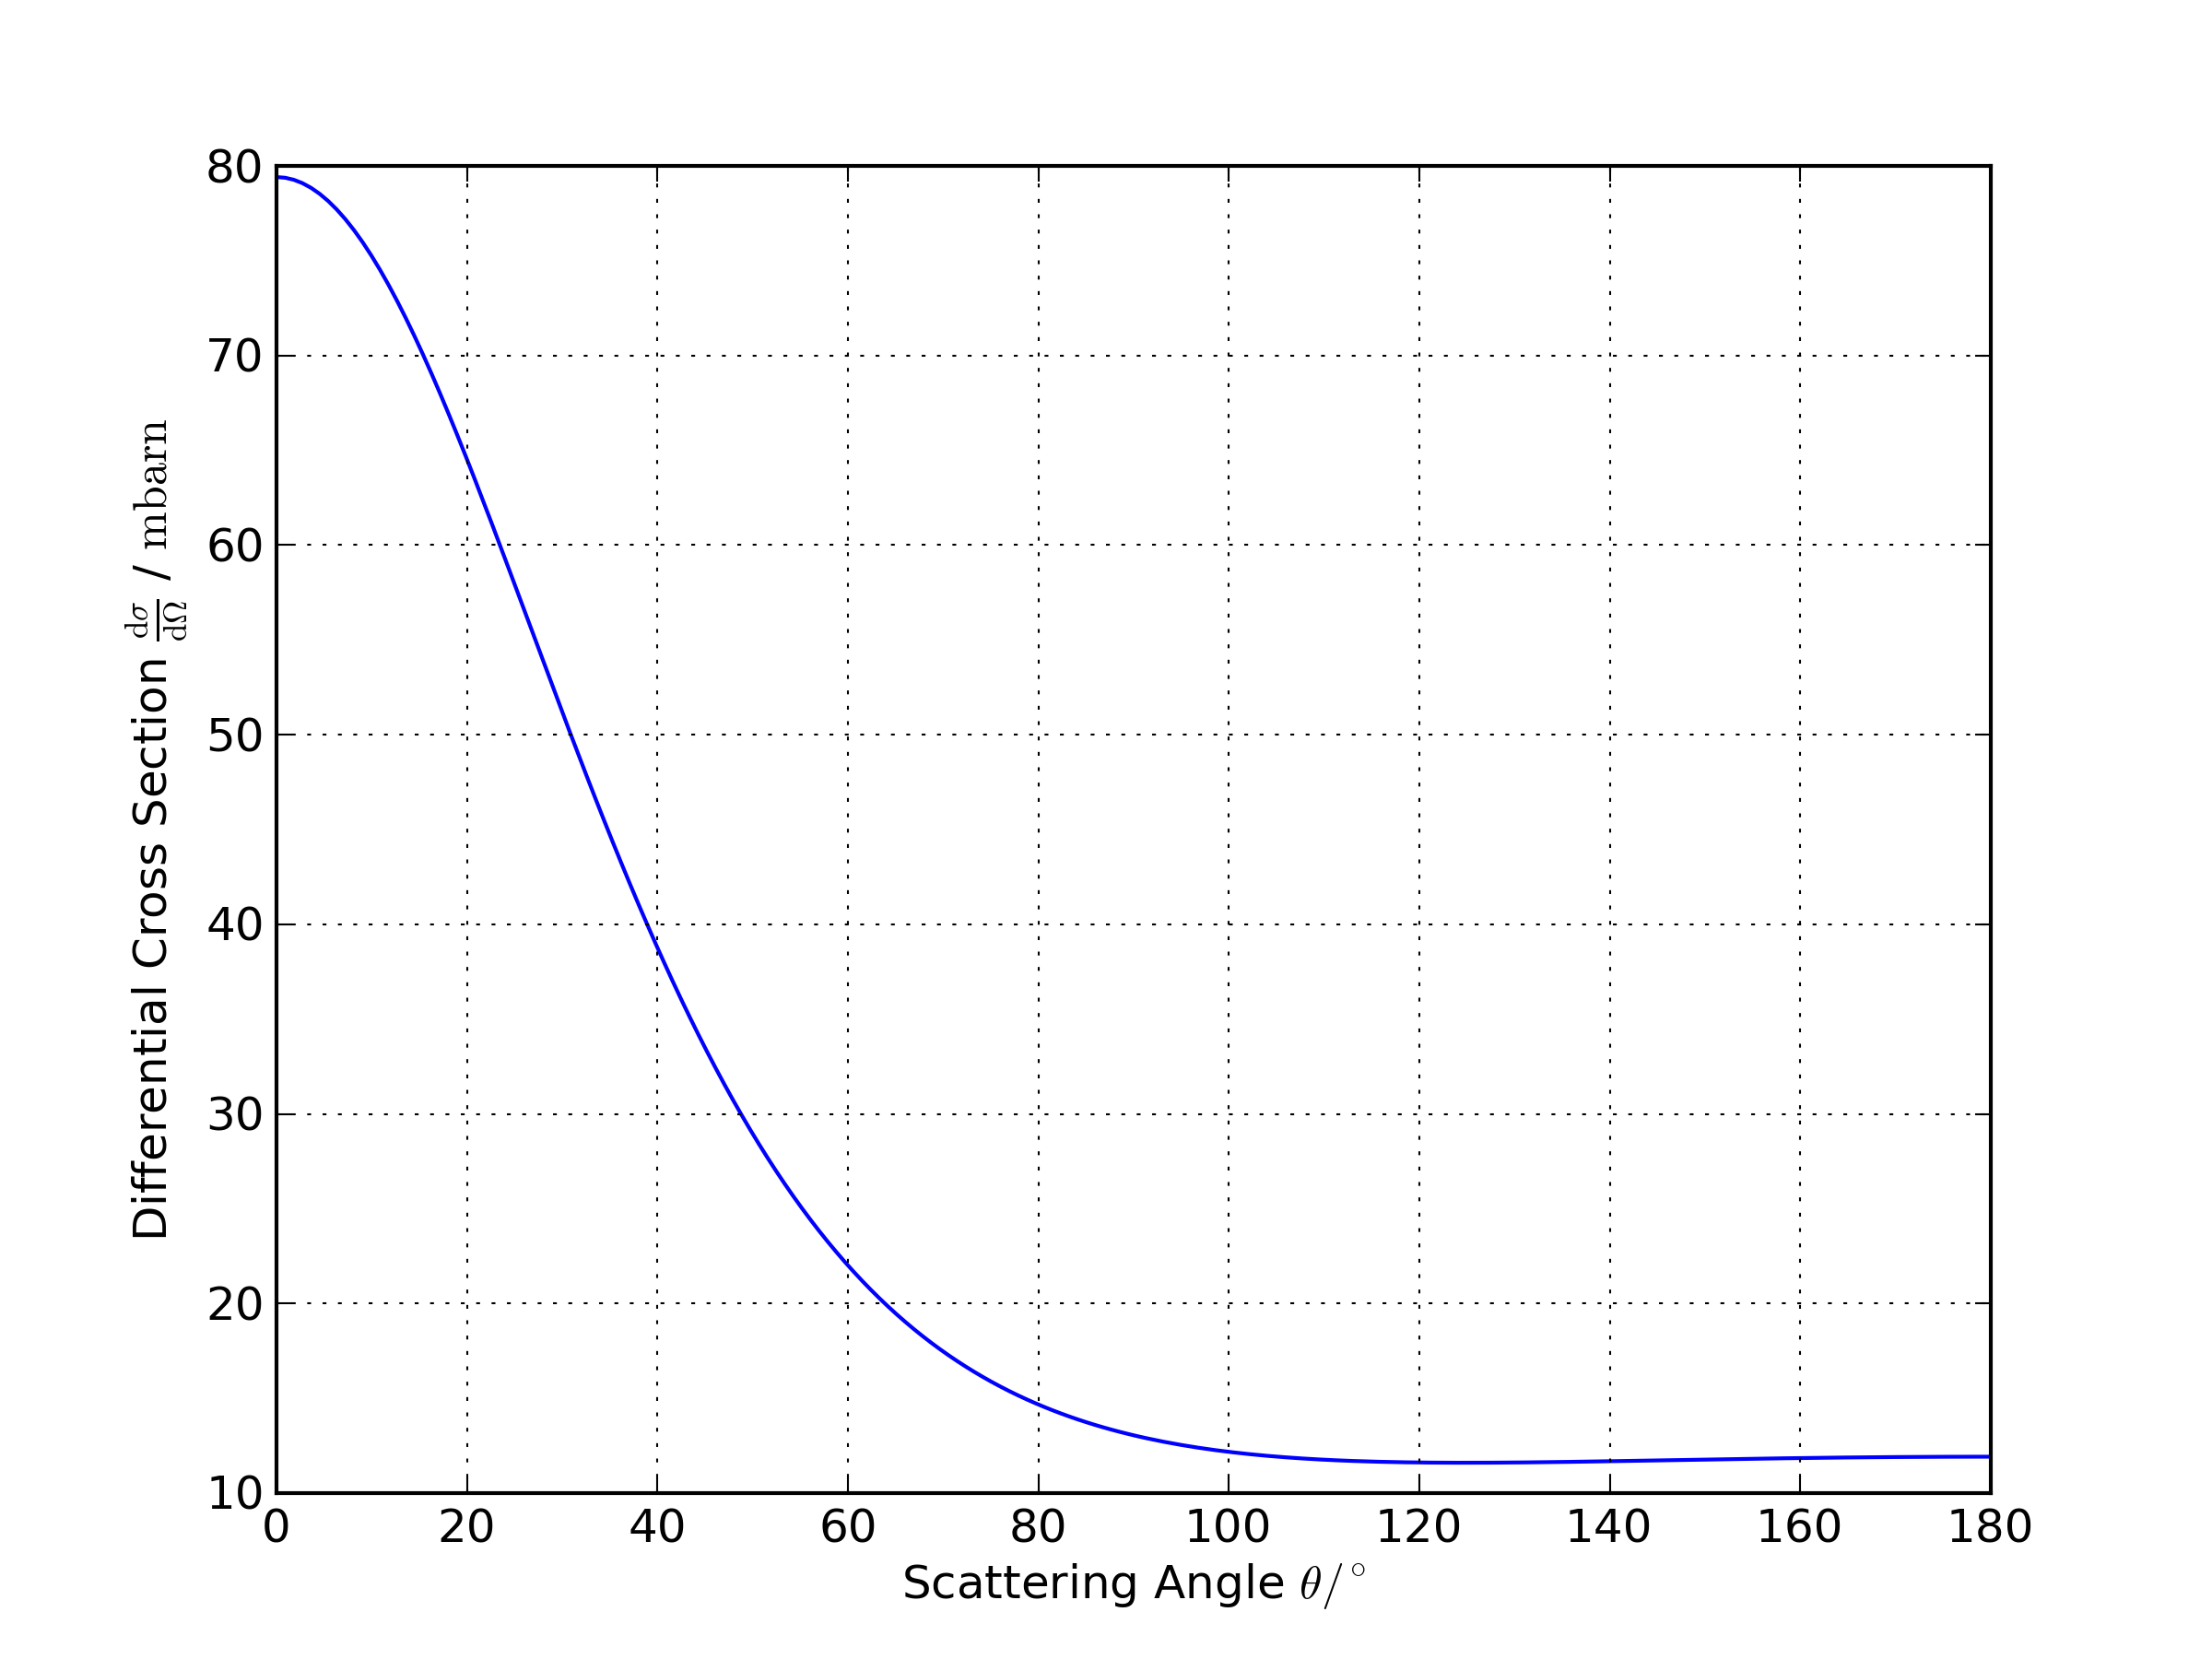
\includegraphics[width=0.9\textwidth]{plots/kleinn.png}
  \caption{Dependence of differential cross section and scattering angle.}
  \label{fig:kleinn}
\end{figure}
